\chapter{Diseño de \maggen}
\label{chap:disen_}
\minitoc

El diseño general de \maggen\ y los diagramas que muestran la arquitectura de la herramienta son presentados en el apéndice \ref{append:disemaggen}. En el desarrollo de este capítulo se presentarán cada una de las capas que conforman a \maggen, mostrando detalles relevantes al diseño. En el siguiente capítulo se analizarán aspectos, correspondientes a cada capa, desde el punto de vista de la implementación.
 
\section{Lenguaje de especificación de las MAG}
\label{sec:lenguajeMAG}

El lenguaje de especificación utilizado para la descripción de una Gramática de atributos (MAG) fue definido en el marco de este proyecto. Este permite definir la entrada de \maggen.
 
La secciones que conforman la descripción de una gramática de atributos (MAG), en el lenguaje, se corresponden con las características que definen una MAG, tal como fueron analizados en los capítulos anteriores (ver capítulo \ref{chap:mag}, principalmente la definición \ref{def:MAG}).
 
Informalmente, el lenguaje de especificación se conforma de las siguientes partes:

\begin{description}
\item [Bloque Dominio Semántico] Destinando a la declaración de sort, operadores y funciones que se utilizarán en los otros dos bloques. Este bloque es denominado ``\textbtt{semantic domain}''.

\item [Bloque de Atributos] Destinando a la declaración y definición de los atributos asociados a cada símbolo. Este bloque es denominado ``\textbtt{attributes}''.

\item [Bloque de Reglas] Destinado a la declaración y definición de las reglas sintácticas de la gramática con sus correspondientes ecuaciones semánticas para cada atributo asociado a cada símbolo. Este bloque es denominado ``\textbtt{rules}''.
\end{description}

Los tres bloques analizados anteriormente, pueden ser clasificados según su comportamiento o funcionalidad dentro del lenguaje la especificación.

Los dos primeros, son bloques puramente declarativos o dedicados a la definición de elementos que serán utilizados en el tercer bloque. La sección de reglas es considerado el de mayor importancia, ya que marca la sintaxis y semántica de la gramática.

Cada bloque del lenguaje de especificación contiene su sintaxis propia para su definición, es por ello que, en las secciones siguientes se mostrarán detalles de cada uno de ellos.

El análisis de cada bloque se realizará de una manera más formal y observando cada bloque como parte de una gramática.

Entonces, sea \textbf{G: CFG} que define el lenguaje de especificación para el archivo de entrada aceptado por \maggen. Se define la siguiente regla de \textbf{G: CFG} para el símbolo inicial ``S''.

\begin{lstlisting}[frame=shadowbox, language=specmag, linewidth=8cm]
S = semantic domain decl_sd
  | attributes decl_attrs
  | rules decl_rules
\end{lstlisting}

En las secciones siguientes se presentarán los símbolos \textit{decl\_Sd}, \textit{decl\_attr} y \textit{decl\_rules} con más detalle.  

\subsection{Bloque Dominio semántico}
\label{subsec:bloq-sem}
El bloque ``\textbtt{semantic domain}'' es el encargado de la definición de elementos que serán necesarios para los bloques siguientes, el mismo esta subdividido en 3 secciones, que se corresponden con la definición de sorts, operadores y funciones, cada una con su sintaxis propia. 

Entonces se define el símbolo \textit{decl\_Sd} como:

\begin{lstlisting}[frame=shadowbox, language=specmag, linewidth=8cm]
decl_sd = (decl_sort)*
        | (decl_operator)*
        | (decl_function)*
\end{lstlisting}

El uso de ``\textbtt{*}'' (``0 o más veces'') en cada subsección y no de ``\textbtt{+}'', esta dado, debido a que cada una de estas secciones son opcionales, es decir, no se obliga a la existencia de cada sección. Por ejemplo, podría interesar la definición de una gramática que no cuente con funciones.

La sintaxis particular de cada sección se analiza individualmente a continuación.

\subsubsection{Declaración de sort}
La subsección de ``\textbtt{sort}'' declara todos los posibles tipos que serán necesarios para las declaraciones siguientes. Todo \textbtt{sort} es distinguible en el lenguaje mediante un nombre.

A continuación se define el símbolo \textbtt{decl\_sort}

\begin{lstlisting}[frame=shadowbox, language=specmag, linewidth=8cm]
decl_sort = sort NAME_SORT  list_sort;

list_sort = , NAME_SORT list_sort
          | `$\lambda$`
\end{lstlisting}

\textit{``NAME\_SORT''} representa el nombre del sort o tipo. El mismo, se corres\-ponde con la definición de un identificador en el común de los lenguajes de programación. Es decir, acepta caracteres alfanuméricos y guiones bajos, restringiendo a los caracteres numéricos como primer carácter, como también palabras reservadas definidas por la especificación (para más detalles ver Apéndice \ref{append:grammarspirit} de implementación en \spirit).\\

\underline{Ejemplo:} \begin{center} \fbox{\textbtt{\ sort fecha;\ }} \end{center}
\vspace{0.2cm}
Esta línea declara el tipo ``\textbtt{fecha}''.

\subsubsection{Tipos predefinidos por el lenguaje}
\label{sec:typepredefined}

El lenguaje de especificación contempla los siguiente tipos básicos:

\begin{description}
\item [int] Tipo entero de 32 bits.

\item [float] Tipo real en punto flotante de 32 bits.

\item [bool] Tiene en cuenta los valores \textbtt{true} y \textbtt{false}.

\item [char] Tipo char en el común de los lenguajes (encerrado entre comillas simples).

\item [string] Cadenas de caracteres (entre comillas dobles).
\end{description}

En caso de declaración explícita de cualquiera de ellos, en la especificación, se informa el error de parser correspondientes, debido a que son consideradas palabras reservadas de \maggen.

\subsubsection{Declaración de operadores}
La sección destinada a la declaración de \textbtt{operadores} acepta 3 tipos de o\-peradores, los cuales, difieren en su forma de uso y cantidad de operandos. Denominados, \textit{infijo, prefijo y posfijo}. 

La interpretación de cada uno, esta dada por la interpretación natural común a todos los lenguajes de programación, a modo de ejemplo se muestran un operador de cada tipo para evitar inconsistencias en las definiciones:

\begin{itemize}
\item \underline{Operador \textbtt{prefijo}:} \textit{Ejemplo:} \textbf{-2}. Operador de menos unario. 

\item \underline{Operador \textbtt{posfijo}:} \textit{Ejemplo:} \textbf{i++}. Operador de auto-incremento en lenguaje C y C++.

\item \underline{Operador \textbtt{infijo}:} \textit{Ejemplo: \textbf{2 + 3}}. Operador ``suma''.
\end{itemize}

A continuación se define el símbolo \textbtt{decl\_operator}:

\begin{lstlisting}[frame=shadowbox, language=specmag, linewidth=11cm]
decl_operator = op infix  mode_op NAME_OP:
                NAME_SORT ,  NAME_SORT -> NAME_SORT;
              | op prefix mode_op NAME_OP:
                NAME_SORT -> NAME_SORT;
              | op postfix mode_op NAME_OP:
                NAME_SORT -> NAME_SORT;
              | op mode_op NAME_OP:
                NAME_SORT -> NAME_SORT;

mode_op = ( m_op )
        | `$\lambda$`

m_op    = NUM_PRECEDENCE , assoc
        | _ , assoc
        | NUM_PRECEDENCE , _
        | _ , _

assoc   = (left | right | non_assoc)
\end{lstlisting}

\textit{``NAME\_OP''} representa un identificador para el operador (infijo, prefijo y posfijo). Las restricciones y detalles a tener en cuenta para este identificador son las mismas que se analizaron para ``NAME\_SORT''.

\textit{``NUM\_PRECEDENCE''} representa un número positivo que define la precedencia del operador. Cabe aclarar que a mayor número mayor la precedencia.

\subsubsection*{Consideraciones}
\label{subsubsec:operconsi}

Es importante analizar el uso de ``\_'' para precedencia y asociatividad, en el hecho de que estos datos son tomados opcionalmente, es decir se puede omitir dicha información. Lo mismo sucede con el tipo del operador (infijo, prefijo y posfijo). 

Para estos casos especiales se utilizarán los siguientes valores por defecto:

\begin{description}
\label{desc:default}
\item [Precedencia] = \textbtt{USHRT\_MAX}.

\item [Asociatividad] = \textbtt{left}.

\item [Tipo de operador] = \textbtt{prefix}.
\end{description}

Otro caso a tener cuenta es el uso de \textbtt{non\_assoc} como asociatividad del operador. Este caso define que el operador no tiene asociatividad, con lo que el uso del mismo en las ecuaciones debe respetar esta condición, en caso contrario se observará un error por mal uso.

\subsection*{Ejemplos}

\begin{enumerate}

\item 
% \begin{center}
\fbox{\textbtt{\ op infix (\_,right) *: int, int -> int;\ }}
% \end{center}
\vspace{0.2cm}
Esta línea declara el operador infijo ``\textbtt{*}'' con precedencia por defecto y asociatividad \textbtt{right}. Esta línea también podría haber sido definida como:
\vspace{0.2cm}
\begin{center}
\fbox{\textbtt{\ op infix *: int, int -> int;\ }}
\end{center}
\vspace{0.2cm}
donde se usan valores por defecto para precedencia y asociatividad.

\item 
% \begin{center}
\fbox{\textbtt{\ op prefix (60,non\_assoc) \%: int -> int;\ }}
% \end{center}
\vspace{0.2cm}
Esta línea declara el operador prefijo ``\textbtt{\%}'' con precedencia \textbtt{60} y asociatividad \textbtt{non\_assoc}. Esta línea también podría haber sido definida como:
\vspace{0.2cm}

\begin{center}
\fbox{\textbtt{\ op (60, non\_assoc) \%: int -> int;\ }}\end{center}
\vspace{0.2cm}
y en el caso que se desee usar valores de asociatividad y precedencia por defecto así:
\vspace{0.2cm}

\begin{center}
\fbox{\textbtt{\ op \%: int -> int;\ }}\end{center}
\end{enumerate}
\subsubsection{Declaración de funciones}
La noción de funciones dentro de la especificación es tomada con la noción natural de función matemática. Es decir, toda función esta definida mediante un identificador, un dominio y una imagen.

Se define \textbtt{decl\_function} como:

\begin{lstlisting}[frame=shadowbox, language=specmag, linewidth=13cm]
decl_function = function NAME_FUNC: decl_domain -> NAME_SORT;

decl_domain = NAME_SORT, decl_domain
            | NAME_SORT
            | `$\lambda$`
\end{lstlisting}

\textit{``NAME\_FUNC''} define el identificador de la función, en el cual se asumen las mismas restricciones tomadas para los identificadores analizados en las secciones anteriores. Cabe aclarar que se acepta un dominio vacío lo que permite el uso de funciones que solo retornan un valor.

Es importante tener en cuenta que las funciones son tomadas con los valores por defecto de operador para asociatividad y precedencia \ref{desc:default}.\\

\underline{Ejemplo:}\ \begin{center}
\fbox{\textbtt{\ function f:int, int, int, int -> real;\ }}                                                                           \end{center}
\vspace{0.2cm}
Esta línea declara la función ``\textbtt{f}'' que tiene como entrada 4 elementos de tipo ``\textbtt{int}'' y como salida un elemento de tipo ``\textbtt{real}''.

\subsection{Bloque de Atributos}
En esta sección se presentará el bloque ``attributes'' en detalle. La información que define un atributo dentro del lenguaje esta dado por: 

\begin{description}
\item [Nombre:] representa el nombre del atributo, el mismo respeta los requisitos de identificador analizados anteriormente.

\item [Clase de atributo:] está dado por la clase del atributo, esto es sintetizado (\textbtt{syn}) o heredado (\textbtt{inh}).

\item [Tipo:] está dado por el tipo del atributo. El mismo corresponde a un tipo básico (ver \ref{sec:typepredefined}) o a un sort definido en la sección de \textit{Sort}.

\item [Símbolos de pertenencia:] hace referencia a los símbolos a los cuales se asocia el atributo.
\end{description}

A continuación se define el símbolo \textbtt{decl\_attrs} como:

\begin{lstlisting}[frame=shadowbox, language=specmag, linewidth=11cm]
decl_attrs = (d_attr)+

d_attr = NAME_ATTR : < c_attr > NAME_SORT of symbols;

symbols = { list_symbol }
        | all
        | all - { list_symbol }

c_attr = inh
       | syn
       | `$\lambda$`

list_symbol = SYMB_NON_TERMINAL , list_symbol
            | SYMB_NON_TERMINAL 
\end{lstlisting}

\textit{``NAME\_ATTR''} define el identificador de un atributo. Se tienen las mismas consideraciones que para el identificador de sort, operador y función.

\textit{``SYMB\_NON\_TERMINAL''} describe un símbolo no terminal de la gramática. En este punto se debe tener en cuenta que los símbolos utilizados deben ser símbolos no terminales utilizados en el bloque de reglas.

\textit{``NAME\_SORT''} declara el tipo del atributo, el mismo esta dado por un sort definido por el usuario o por un tipo predefinido por el lenguaje \ref{sec:typepredefined}.

\subsubsection*{Consideraciones}

\begin{itemize}
\item En la declaración de los símbolos a los cuales pertenece el atributos, ``\textbtt{all}'' se interpreta como ``todos los símbolos'', es decir, el atributo declarado se asocia a todos los símbolos de la gramática. Además es posible utilizar el operado ``diferencia'' de conjuntos ``\textbtt{-}'' para especificar el conjunto de símbolos a los cuales perteneces el atributo, como una expresión.

\item Si no se especifica la clase del atributo (sintetizado o heredado) el mismo es tomado como el caso por defecto a sintetizado.
\end{itemize}

\subsection*{Ejemplos}
\begin{enumerate}

\item 
% \begin{center}
\fbox{\textbtt{\ lex: syn <string>\ of all - {T};\ }}
% \end{center}
\vspace{0.2cm}
Se define el atributo ``\textbtt{lex}'' sintetizado de tipo ``\textbtt{string}'' para todos los símbolos excepto para el símbolo ``\textbtt{T}''.

\item
% \begin{center}
\fbox{\textbtt{\ type: inh <string>\ of all;\ }}
% \end{center}
\vspace{0.2cm}
Se define el atributo ``\textbtt{type}'' heredado de tipo ``\textbtt{string}'' para todos los símbolos de la gramática.

\item 
% \begin{center}
\fbox{\textbtt{\ grade: <int>\ of {E, T};\ }}
% \end{center}
\vspace{0.2cm}
Se define el atributo ``\textbtt{grade}'' sintetizado (por defecto) de tipo ``\textbtt{int}'' para los símbolos ``\textbtt{E}'' y ``\textbtt{T}''.\\
\end{enumerate}

\subsection{Bloque de reglas}
Por último el bloque de reglas. La interpretación de las reglas dentro del lenguaje esta dada por la definición de gramática libre de contexto (Ver definición \ref{sec:def-CFG}).          

El símbolo terminal se considera un símbolo entre comillas simples (\textbtt{'}).

\underline{Ejemplo:}
\vspace{0.2cm}
\begin{center}
\fbox{\ \textbtt{'literal'}\ }\\
\end{center}
\vspace{0.2cm}

Las ecuaciones describen las reglas semánticas que definen la sintaxis de la gramática. Cada ecuación define la interpretación semántica de los atributos de cada símbolo; esta definición se realiza mediante una expresión constituida por \textbf{instancias}, \textbf{literales} o aplicación de operadores y funciones a subexpresiones.
En este punto se deben tener en cuenta los requisitos necesarios de una gramática bien definida (Ver sección \ref{sec:well-defined}).

A continuación se define el símbolo \textbtt{decl\_rules}:

\begin{lstlisting}[frame=shadowbox, language=specmag, linewidth=11cm]
decl_rules = (d_rule)+ 

d_rule = SYMB_NON_TERMINAL ::= rigft_symb decl_eqs

rigft_symb = (SYMB_NON_TERMINAL | SYMB_TERMINAL)+

decl_eqs = compute d_eqs end;
         | ;

d_eqs = instance = right_eq;

right_eq = leaf
         | leaf OP_NAME leaf right_eq
         | (OP_NAME)+ leaf
         | leaf (OP_NAME)+
         | NAME_FUNC ( right_eq ) 

leaf = instance
     | LITERAL

instance = SYMB_NON_TERMINAL[NUM_INS].NAME_ATTR
\end{lstlisting}

\textit{``SYMB\_NON\_TERMINAL''} y \textit{``SYMB\_TERMINAL''} describen símbolos no terminales y terminales respectivamente. En este punto, se tiene en cuenta la diferenciación entre estos tipos de símbolos como se analizó en el párrafo anterior (a través de \' para los terminales).
 
\textit{``OP\_NAME''} y  \textit{``NAME\_FUNC''} describen identificadores de operadores infijos, prefijos y posfijos (según su uso) y el de función respectivamente. Tanto los operadores como las funciones se asumen definidos en la sección ``\textbtt{semantic domain}''.

\textit{``NUM\_INS''} corresponde con un número mayor que cero que identifica la ocurrencia del símbolo (para más detalle ver \ref{subsec:consirule} punto 4).

\textit{``LITERAL''} describe los tipos de literales entero, real, carácter, string y bool con las siguientes consideraciones:

\begin{description}
\item [Entero] es considerado un número entero de 32 bits. 
\item [Real] es considerado un número en punto flotante de 32 bits. La separación de decimales se da mediante el punto (.).
\item [Carácter] es considerado un carácter cualquiera entre comillas simples (').
\item [String] es considerado una cadena de caracteres entre comillas dobles (`` '').
\item [Bool] representa los valores \textbtt{true} y \textbtt{false}.
\end{description}

\subsubsection*{Consideraciones}
\label{subsec:consirule}
\begin{enumerate}
\item Es posible definir una regla de la gramática sin sección de ecuaciones, para ello se debe omitir la sección de ``\textbtt{compute}'' en la definición. Si se define la sección de ``\textbtt{compute}'' el lenguaje obliga a definir \textbf{al menos una ecuación}.

\item La sintaxis para el uso de los operadores esta dada por el tipo del operador: infijo, prefijo o posfijo. Para las funciones se utiliza la manera natural de invocación de una función en el común de los lenguajes de programación. Esto es, mediante el nombre de la función y los parámetros entre paréntesis.

\item La asociatividad y precedencia de la expresión en las ecuaciones es calculada mediante los valores definidos en las sección de declaración de funciones. Cabe aclarar que es posible utilizar paréntesis para agrupar subexpresiones.

\item La asociación del símbolo no terminal con el atributo se denomina \textbf{instancia}. La misma se corresponde con la \textit{ocurrencia del símbolo}\footnote{El concepto de ocurrencia de un símbolo fue presentado en el capítulo introductorio en la definción \ref{def:grammarattr}}. 

Se compone de tres partes\footnote{Estas partes se corresponden con las usadas para el desarrollo de \maggen.}:
\begin{itemize}
\item Símbolo no terminal.
\item Índice sintáctico, comenzando de 0 para la primera ocurrencia.
\item Atributo.
\end{itemize}
\underline{Ejemplo:}
\vspace{0.2cm}
\begin{center}
\fbox{\ \textbtt{E[2].type}\ }
\end{center} 

Asocia al símbolo ``E'' con el atributo ``type'' en la ocurrencia 3 del símbolo.

\end{enumerate}

\subsubsection*{Ejemplos}
\begin{enumerate}

\item 
\fbox{\ E ::= E '+' E \ compute\ 
                       E[0].valor = E[1].valor + E[2].valor; 
                       end;\ }

El ejemplo muestra una regla del símbolo ``\textbtt{E}'' que contiene una ecuación que define al atributo sintetizado \textbtt{valor}, asumiendo que no tiene atributos heredados. Si se considera, una ``Gramática Bien Definida'' (Ver \ref{sec:well-defined}), \textbtt{valor} es un atributo sintetizado de ``\textbtt{E}''. Otra consideración a tener en cuenta, es la enumeración sintáctica de cada símbolo; en este ejemplo cada símbolo ``\textbtt{E}'' presenta su índice sintáctico que asocia a los atributos con cada símbolo. Es decir, cada símbolo ``\textbtt{E}'' es reconocido como un nuevo símbolo. A modo de aclaración, se podría definir la ecuación de la siguiente, obteniendo el mismo poder expresivo para la regla:
\begin{center}
\fbox{\ E ::= T '+' F \ compute\ 
      E[0].valor = T[0].valor + F[0].valor; 
      end;\ }
\end{center}

Cabe aclarar que \textbtt{valor} debe ser atributo de ``\textbtt{T}'' y ``\textbtt{F}''.
\vspace{0.2cm}

\item
\fbox{\ \textbtt{digit ::= '1';}\ }

Se observa una regla para el símbolo no terminal ``\textbtt{digit}'' sin ecuaciones semánticas. 
\vspace{0.2cm}
\end{enumerate}

\subsection{Comentarios}

La especificación permite agregar comentarios. Para una mejor familiarización con el usuario se han utilizado las mismas reglas sintácticas que C y C++ para el adicionado de líneas o bloques de comentarios. Las cuales se detallan a continuación:

\begin{description}
\item [$\textbf{/*}$ comment $\textbf{*/}$] Forma de inserción de bloques de comentarios.
\item [$\textbf{//}$ line comment] Comentario de una línea.
\end{description} 

\subsection{Ejemplo}

En el apéndice \ref{append:agwuuyang} se puede observar uno de los casos de prueba desarrollado para la fase de testing de \maggen. El mismo es presentado en pseudocódigo y luego escrito en el lenguaje de especificación. 

Una característica que motivó el desarrollo de este ejemplo es que se trata de una gramática \textbf{MAG} pero no \textbf{ANCAG}. Además, el mismo, es un caso de estudio analizado en una de las principales bases teóricas que han sido usadas para el desarrollo de \maggen\ (\cite{wuu-yang1}). 

En la presentación del ejemplo en el lenguaje de especificación, se observa en principio (línea 1 a 7) un bloque de comentario y luego los bloques que definen la gramática como se ha analizado en las secciones anteriores; bloque semántico de la línea 8 a 13 luego el de atributos y a partir de la línea 25 el bloque de reglas con sus respectivas ecuaciones.

 
\section{Parser del lenguaje, representación interna y chequeos}

El parser del lenguaje de especificación se llevó a cabo utilizando las librerías \boost\ \spirit. Detalles de este tema, son tratados puntualmente en las secciones \ref{sec:par-spirit} y \ref{sec:gramspirit}. 

En esta sección se mencionarán algunas consideraciones sobre el parser desde el punto de vista de su funcionamiento, detalles en la representación interna y los chequeos realizados sobre la entrada de \maggen, para asegurar y verificar que se cumpla las características de una ``Gramática Bien Definida''.

\subsection{Parser del lenguaje}
\label{subsec:parsers-leng}
El parser de la entrada de \maggen\ esta dado por un recorrido secuencial y ante cualquier error sintáctico, la herramienta finaliza su ejecución indicando el error correspondiente. 

Si se supone la siguiente porción de especificación de una entrada de \maggen:

\begin{lstlisting}[numbers=left, firstnumber=9, language=specmag, linewidth=8cm, columns=fullflexible]
...
semantic domain
  sort ecuacion, lista;

  /* List of Operators */
  op infix    10, left) +: int, int -> int;
...
\end{lstlisting}

La línea 15 presenta un error de sintaxis (falta de paréntesis), entonces \maggen\ finaliza el parser e informa de la siguiente manera:

\begin{lstlisting}[backgroundcolor=\color{white}, language=]
   * Parsing grammar ---------- [ FAIL ]

   ERROR: Parsing Failed, the following text will not be able to parse:

   File: ./examples/ag_count/ag_count.input
   Line: 17
   Col:  5
\end{lstlisting}

Notar que, la línea y columna donde se indica el error corresponde al inicio de la zona donde la interpretación fue fallida. Podría suceder en varios casos que el error no se detecte específicamente en la línea y columna que se indica, entonces lo conveniente es buscar el error a partir del punto especificado. Para este caso particular, se indica línea: 17 y columna: 5, este punto se encuentra sobre \textbtt{op}, pero el error se observa seguido de \textbtt{infix}.

\subsection{Representación interna}

Las estructuras creadas para la representación interna de la gramática se encuentran dentro de los paquetes \textbtt{Attr\_grammar} y \textbtt{Expression\_tree} de \maggen. Detalles de implementación sobre estos paquete serán tratando en el capítulo siguiente. 

Ahora se presentarán detalles respecto al diseño.
\textbtt{Expression\_tree} agrupa módulos para la representación de las expresiones de las ecuaciones y \textbtt{Attr\_grammar}, encapsula los demás componentes de la gramática.

El funcionamiento de \maggen\ esta dado por una instancia de la estructura llamada \textbtt{Attr\_grammar}, la cual encapsula toda la información de la gramática de atributos parseada. La misma contiene los elementos que se agrupan en los paquetes anteriormente nombrados y es la que desencadena el cálculo de planes, secuencias de visita y, por último, la generación de código. 
 
En la figura \ref{fig:disen} se presenta un diagrama que muestra la interacción de esta estructura en el funcionamiento de \maggen.

\begin{figure}[!ht]\centering
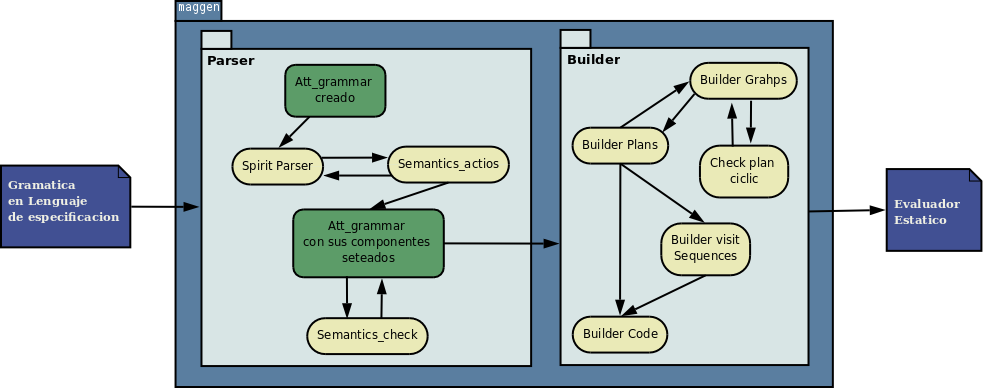
\includegraphics[width=400pt,height=158pt]{Disen.png}
\caption{\label{fig:disen}Interacción de Attr\_grammar en \maggen}
\end{figure}

A continuación se analizan cuestiones de diseño de los paquetes mencionados arriba, y con ellos la estructura \textbtt{Attr\_grammar}.  En la figura \ref{fig:disen2} se muestra un diagrama con la representación interna de una gramática dentro de \maggen.

\begin{figure}[!ht]\centering
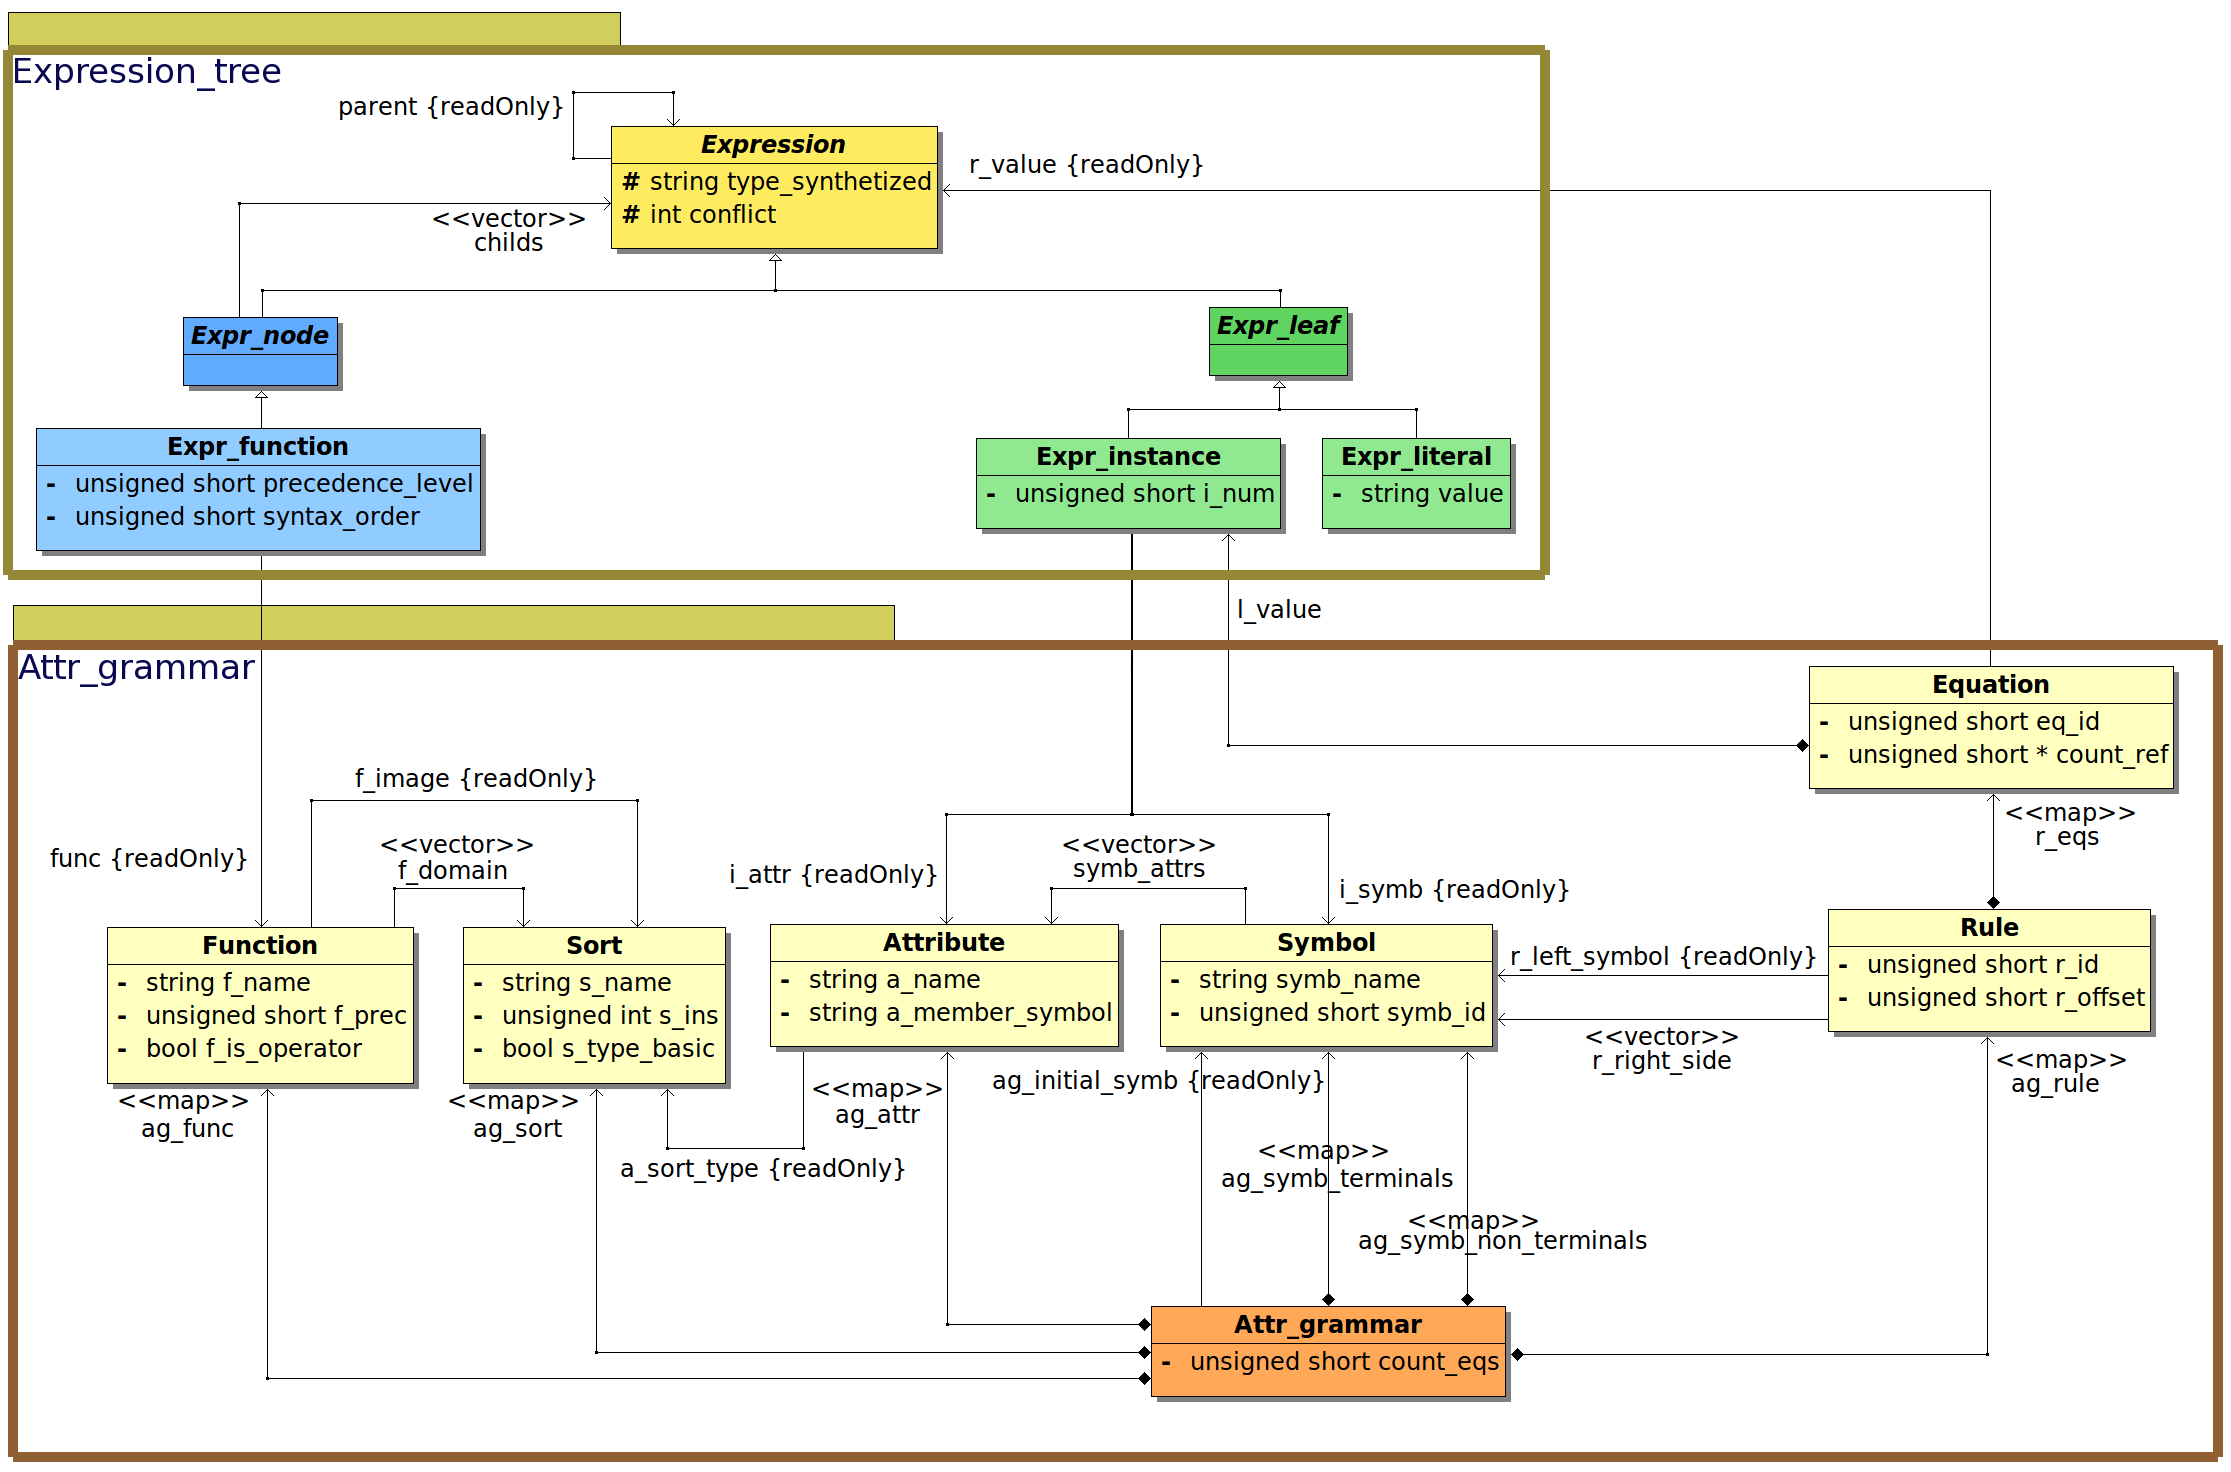
\includegraphics[width=400pt,height=264pt]{Disen2.png}
\caption{\label{fig:disen2}Diseño interno de una gramática de atributos en \maggen}
\end{figure}

Algunas observaciones sobre el diseño realizado en la figura \ref{fig:disen2}:

\begin{itemize}
\item La relación entre los paquetes se produce por un lado, mediante la clase \textbtt{Rule}, en el sentido de que toda regla contiene un conjunto de ecuaciones y cada una de estas, está definida a través de un \textit{l\_value:} \textbtt{Expr\_instance} y un \textit{r\_value:} \textbtt{Expression}. Por otro lado, \textbtt{Expr\_instance} se vincula con \textbtt{Symbol} y \textbtt{Attribute} y \textbtt{Expr\_function} con \textbtt{Function}.

\item Toda la información de una gramática de atributos esta representada en la clase \textbtt{Attr\_grammar} y por ende, el ciclo de vida de cada uno de sus componentes es administrado por esta clase, durante todo el funcionamiento de \maggen. 
\end{itemize}

\subsection{Chequeos}
\label{subsec:check}

El conjunto de chequeos que se realizan sobre la gramática de entrada a \maggen, están directamente relacionados con el concepto de gramática bien definida analizado en la sección \ref{sec:well-defined}. Además, se aplican una serie de chequeos extras para evitar cálculos inconsistentes en las etapas posteriores. La totalidad de los chequeos, son realizados sobre el bloque de reglas de la gramática\footnote{En su mayoría los chequeos se realizan sobre las ecuaciones de las reglas.}, debido a que este, es el más significativo y sobre el cual se apoyan los cálculos posteriores (en particular, el cálculo de planes).

Los chequeos realizados son clasificados en sintácticos y semánticos, los primeros, en su mayoría, son realizados durante el parser, en cambio, los chequeos semánticos se realizan luego de parsear cada regla, aplicando escaneos específicos. Estos últimos son los explicados en esta sección.

El módulo que agrupa estos chequeos, se ubica en el paquete \textbtt{Parser} de \maggen\ y se denomina \textbtt{Semantics\_checks}.

A continuación se detallan dichos chequeos\footnote{Detalles sobre la implementación de cada uno de los chequeos, ver sección \ref{sec:checksem}.}:

\begin{description}
\item [Precedencia] El chequeo de precedencia consiste en preservar la precedencia definida de cada operador. Dicho chequeo, es realizado sobre cada una de las ecuaciones definidas en la gramática. Por ejemplo:\\ Dada la siguiente ecuación:

\begin{center}
 \fbox{\ \textbtt{E[0].valor = E[1].valor + E[2].valor * E[2].valor}\ }
\end{center}

Su interpretación está dada por la definición de la precedencia de los o\-pe\-radores \textbtt{+} y \textbtt{*} (se asume que los dos operadores son infijos y están bien usado). Si se toma \textbtt{*} con mayor precedencia que \textbtt{+}, \maggen\ interpreta implícitamente como si la ecuación tuviera paréntesis:

\begin{center}
 \fbox{\ \textbtt{E[0].valor = E[1].valor + (E[2].valor * E[2].valor)}\ }
\end{center}

El uso de paréntesis en las expresiones define explícitamente la prioridad de los operadores, por lo que, \maggen\ asume esa precedencia. Por ejemplo, si en la ecuación vista arriba se la define utilizando paréntesis, es decir:\  
 \fbox{\ \textbtt{E[0].valor = (E[1].valor + E[2].valor) * E[2].valor}\ }\ la interpretación es tomada en ese sentido.

\item [Asociatividad] El chequeo de asociatividad realiza un análisis sobre las expresiones de las ecuaciones, para asegurar la asociatividad definida de cada operador. Por ejemplo, si se ha definido un operador \textbtt{non\_assoc}, se espera que el uso del mismo sea consistente con esa definición, es decir, no se considere una posible asociación del mismo. 

Cuando se utilizan paréntesis en la expresión, \maggen\ asume la asociatividad que se especifica explícitamente.

\item [Alcanzabilidad] Es una característica importante a tener en cuenta sobre los símbolos de la gramática. Este chequeo, realiza un análisis sobre la totalidad de las reglas en busca de símbolos no terminales no alcanzables desde el símbolo inicial. Este caso no es considerado error fatal en \maggen, sino como \textit{warning}.

\item [Condiciones de AG] Este chequeo tiene en cuenta un conjunto de condiciones que debe cumplir la gramática. Ellos son:

\begin{itemize}
\item Cada regla debe definir todos los atributos sintetizados del símbolo de la parte izquierda.
\item Cada regla debe definir todos los atributos heredados de los símbolos de la parte derecha.
\item Cada regla sólo define los atributos de los símbolos que participan en dicha regla.
\item En caso de redefinición alguna instancia en la regla, la misma es ignorada.
\item Los índices de las instancias deben ser consistentes con la cantidad de apariciones del símbolo en la regla.\\ \underline{\textbf{Ejemplo:}}\\
En la siguiente regla:\ \fbox{\ \textbtt{S ::= S T}\ }\ los índices posibles de las instancias son \textbtt{0} y \textbtt{1} para el símbolo ``\textbtt{S}'' y \textbtt{0} para el símbolo ``\textbtt{T}''.
\item La gramática debe respetar las condiciones exigidas para una gramática extendida. 
\end{itemize}
\end{description}

\section{Construcción de grafos, planes y secuencias de visita}

En la figura \ref{fig:disen} se puede visualizar el funcionamiento de \maggen, teniendo en cuenta la estructura \textbtt{Attr\_grammar}, en esta sección se abordan detalles sobre el diseño del paquete \textbtt{Builder}, específicamente en la construcción de grafos, de planes y de secuencias de visita. Un detalle a tener en cuenta es que, a partir de esta etapa, todas las manipulaciones son realizadas sobre las ecuaciónes de cada regla.

\subsection{Construcción de grafos}
\label{subsec:graph}

Detalles de implementación serán analizados en la sección \ref{subsec:const-graf}, ahora se mencionarán las consideraciones más relevantes con respecto al funcionamiento de los grafos en \maggen.\\

La construcción de grafos se realiza en el módulo \textbtt{builder\_graphs}. \maggen\ crea 4 tipos de grafos, que se corresponden con los detallados en \ref{sec:pre-grafos}:

\begin{itemize}
\item Grafo DP, ver \ref{dpgraph}.
  \begin{figure}[!ht]\centering
    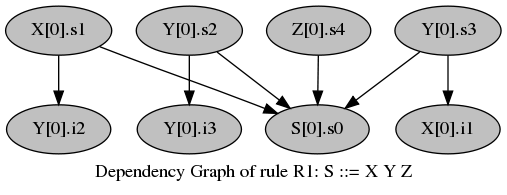
\includegraphics[width=200pt,height=77pt]{graph/dp.png}
  \caption{\label{dpgraph} Grafo DP.}
  \end{figure}

\item Grafo Down, ver \ref{downgraph}.
  \begin{figure}[!ht]\centering
    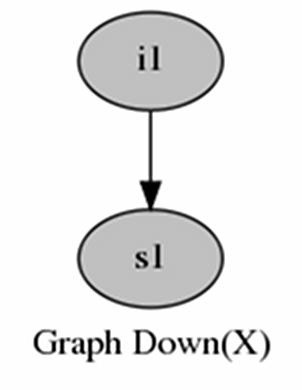
\includegraphics[width=75pt,height=97pt]{graph/down.png}
  \caption{\label{downgraph} Grafo Down.}
  \end{figure}

\item Grafo DCG, ver \ref{dcggraph}.
  \begin{figure}[!ht]\centering
    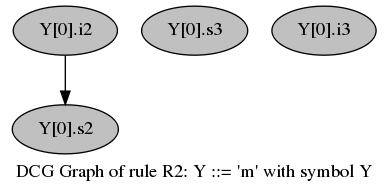
\includegraphics[width=200pt,height=101pt]{graph/dcg.png}
  \caption{\label{dcggraph} Grafo DCG.}
  \end{figure}

\item Grafo ADP, ver \ref{adpgraph}.
  \begin{figure}[!ht]\centering
    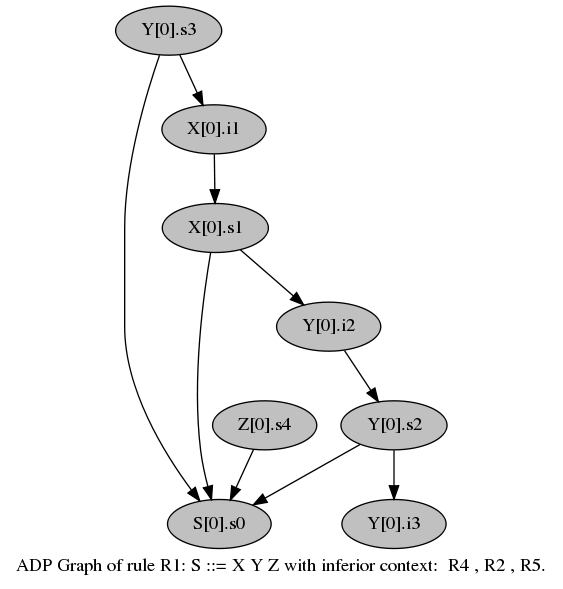
\includegraphics[width=200pt,height=209pt]{graph/adp.png}
  \caption{\label{adpgraph} Grafo ADP.}
  \end{figure}
\end{itemize}

Las figuras\footnote{\label{foot:graph} Imagen generada utilizando la herramienta \textbtt{graphviz} sobre el archivo \textbtt{.dot} generado por \maggen.} muestran un ejemplo de cada tipo de grafo, generadas a partir del ejemplo analizado en el apéndice \ref{append:agwuuyang}.

La construcción de cada tipo de grafo respeta los principios analizados en el capítulo \ref{chap:mag} y los respectivos algoritmos analizados en el capítulo \ref{chap:eval_est}. 

De de los 4 tipos de grafos analizados, los necesarios para el cómputo de etapas siguientes, son los ``\textbtt{ADP graph}''. Los demás, son requeridos como cálculo previo para la construcción de estos.

\subsection{Construcción de planes}
\label{subsec:conts-plan-dise}
La etapa de construcción de planes, tal como lo muestra el diagrama de la figura \ref{fig:disen}, se realiza en el paquete ``\textbtt{Builder}''. El cálculo de planes en \maggen\ se basa en lo analizado en el capítulo \ref{chap:eval_est} (Ver sección \ref{sec:comp-planes}) y teniendo en cuenta estos dos puntos:

\begin{enumerate}
\item El punto de entrada para el cálculo de los planes esta dado sobre los grafos \textbf{ADP}. 
\item El cálculo de planes se basa en un orden topológico de la evaluación de los atributos de los símbolos, teniendo en cuenta los distintos contextos posibles.
\end{enumerate}

En la sección \ref{sec:obtplaneval} se tratan detalles de implementación, en donde se analiza el funcionamiento de lo tratado anteriormente, en especial el punto 2.

Un \textbf{plan} se compone de una lista de números de ecuaciones a computar. Todo plan determina un orden de evaluación, realizándose la evaluación de izquierda a derecha.

\subsubsection{Planes proyectados}

Estos se obtienen a partir de los planes analizados anteriormente, proyectando el plan para cada símbolo de la parte derecha de la regla. La importancia de estos planes radica en la construcción de las secuencias de visita y además en el algoritmo principal de evaluación en la generación de código.

\begin{figure}[!ht]\centering
 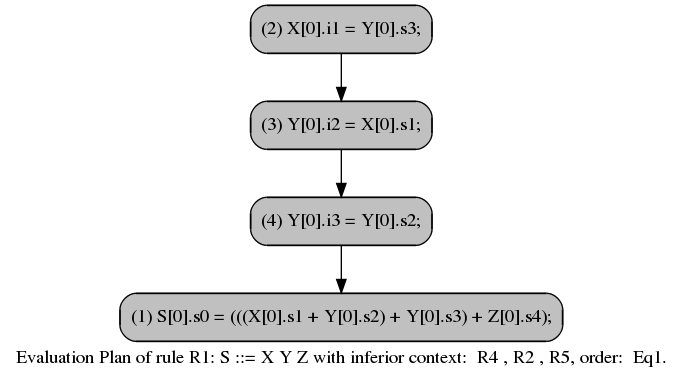
\includegraphics[width=250pt,height=139pt]{plans/plan.png}
\caption{\label{fig:plan}Plan obtenido por \maggen\ para la regla R1}
\end{figure}

En la figura\footnote{Figura obtenida con la herramienta \textbtt{graphviz} sobre el archivo \textbtt{.dot} generado por \maggen.} \ref{fig:plan} se observa un plan obtenido por \maggen\ para el ejemplo del apéndice \ref{append:agwuuyang}. Este plan contiene el orden de los números de ecuación que pertenecen a la regla del plan, los planes proyectados son computados sobre el plan total, es decir con todas las dependencias.

Para clarificar este concepto, se pueden observar los planes proyectados obtenidos en la figura \ref{fig:plan_project}, para el plan de evaluación anterior.

\begin{figure}[!ht]\centering
\begin{tabular}{l l}
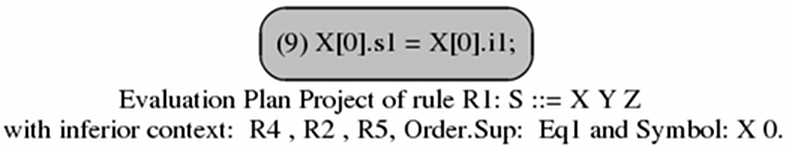
\includegraphics[width=180pt,height=34pt]{plans/plan_proj1.png} &
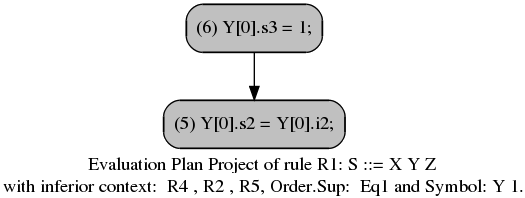
\includegraphics[width=180pt,height=68pt]{plans/plan_proj2.png}\\ 
\multicolumn{2}{c}{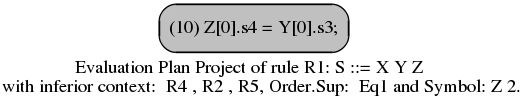
\includegraphics[width=180pt,height=34pt]{plans/plan_proj3.png}}\\
\end{tabular}
\caption{\label{fig:plan_project}Planes proyectados obtenido por \maggen\ para R1.}
\end{figure}

Notar que cada plan proyectado ha capturado las ecuaciones de cada símbolo de la parte derecha para el cómputo de sus atributos, dependiendo del contexto. Es decir, en el caso del símbolo ``\textbtt{Y}'' su orden ha sido computado observando las dependencias de la regla R2. Estas dependencias son necesarias para el cálculo del plan completo en las ecuaciones 2 y 4. 

\subsection{Construcción de secuencias de visita}
\label{sec:constseqvisit}

La etapa de construcción de secuencias de visita, tal como lo muestra el diagrama de la figura \ref{fig:disen}, se realiza en el paquete ``\textbtt{Builder}''. Las mismas, son computadas a partir de los diferentes planes obtenidos en el sección anterior.

El funcionamiento para la construcción de las secuencias, esta dado por la aplicación de un recorrido recursivo sobre los contextos de las reglas, para la evaluación de cada atributo de los símbolos. El resultado de este algoritmo, son los valores que conforman la secuencia de visita, tal como se ha analizado en la sección \ref{sec:sec-visit}. Estos valores tienen la siguiente interpretación: 

\begin{description}
\item [Compute] Valor menor que cero que representa el número de la ecuación a resolver\footnote{La ecuación a computar pertenece a la regla del plan corriente.}.
\item [Visit] valor mayor que cero que representa el número nodo hijo a visitar\footnote{El nodo hijo esta dado por el contexto de la regla del plan corriente.}.
\item [Leave] valor ``\textbtt{0}''.
\end{description}

A modo de ejemplo, se muestran las secuencias de visita generadas por \maggen\ para el ejemplo analizado en el apéndice \ref{append:agwuuyang}:

\begin{description}
\item [\{-7,0,-8\}] Secuencia de visita para la regla \textbtt{R3} (sin contexto inferior). En este caso, la secuencia de visita se traduce a lo siguiente:

\begin{enumerate}
\item \textbf{Computar} la ecuación 7.
\item \textbf{Leave}\footnote{El leave retorna el control a la secuencia de visita de contexto superior, es decir, desde donde se invocó a esta secuencia.}.
\item \textbf{Computar} la ecuación 8.
\end{enumerate}

\item [\{-11,1,-12,-10\}] Secuencia de visita para la regla \textbtt{R5} con el contexto de \textbtt{P2}. En este caso, la secuencia de visita se traduce a lo siguiente:

\begin{enumerate}
\item \textbf{Computar} la ecuación 11.
\item \textbf{Visitar} el nodo hijo 1, es decir \textbtt{Y}, como el contexto es \textbtt{P2}, significa visitar a R2.
\item \textbf{Computar} la ecuación 12.
\item \textbf{Computar} la ecuación 10.
\end{enumerate}
\end{description}

Cabe aclarar que todas las secuencias de visita tienen un \textbf{leave} implícito al final, es decir, cuando se completó la computación de la secuencia se retorna a su ámbito de invocación.

\subsubsection{Heurística del algoritmo}
\label{subsec:heuris-simul}
El punto principal en el cual se basa la heurística, es evaluar el plan buscando las dependencias de cada ecuación en el contexto del mismo. A continuación se muestran los pasos básicos a tener en cuenta con un ejemplo:\\

Si se toma uno de los planes\footnote{Es importante notar el hecho de que cada plan se conforma de los números de ecuaciones a computar.} calculados por \maggen\ para el ejemplo del apéndice \ref{append:agwuuyang}:\\

\underline{Plan:} \{ 2, 3, 4, 1 \}. Ver figura \ref{fig:plan}.

\begin{enumerate}
\item Se recorre el plan tomando en cada paso una de las ecuaciones. Para este caso particular se comienza con la ecuación 2.

\item Dada la ecuación \textbtt{i}\footnote{Para este caso particular \textit{i} toma los valores 1,2,3,4.}, en el plan, se debe computar todo el \textit{l\_value} de la ecuación. Para ello se deben resolver todas las dependencias dadas por \textit{r\_value}.

\item Dada una dependencia de la ecuación, primero se chequea si la misma fue computada en algún paso anterior, sino, se analizan los siguientes casos:

\begin{itemize}
\item Si la dependencia proviene de una instancia que pertenece al \textbf{símbolo de la parte izquierda de la regla} y además contiene un \textbf{atributo heredado}, entonces se debe realizar un ``\textbtt{leave}''.

\item Si la dependencia proviene de una instancia que pertenece a un \textbf{símbolo de la parte derecha de la regla} y además contiene un \textbf{atributo sintetizado}, entonces se debe de realizar un ``\textbtt{visit}''. En este caso, se debe analizar, según el contexto, cuál es el plan se debe visitar, es decir, a cuál nodo hijo. 
\end{itemize}

Notar que en los dos puntos anteriores, no se incluyen los casos de dependencia perteneciente al símbolo de la parte izquierda con atributo sintetizado y dependencia de símbolo de la parte derecha con atributo heredado, pero estos casos, son los que deben definirse en este ambiente y como se parte del plan evaluación, el orden de dependencias es consistente con la demanda de las mismas.

\item Luego de la obtención de todas las dependencias, se realiza un \textbf{compute} del \textit{l\_value} y se marca a este como \textbtt{evaluado}. El paso siguiente es avanzar una ecuación en la lista que impone el plan y realizar los mismos tratamientos.
\end{enumerate} 

Para más detalle en la figura \ref{fig:simul} se grafica este proceso.

\begin{figure}[!ht]\centering
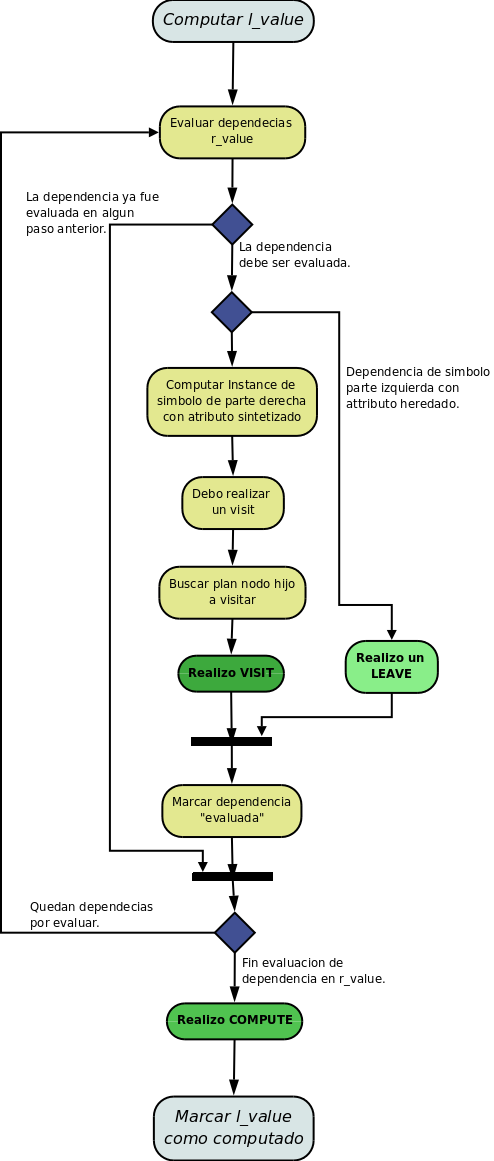
\includegraphics[width=228pt,height=400pt]{simu.png}
\caption{\label{fig:simul}Heurística cómputo de secuencia de visita}
\end{figure}

El resultado del ejemplo, aplicando los pasos tratados arriba, es presentado en el diagrama \ref{fig:resul_vis}.

\begin{figure}[!ht]\centering
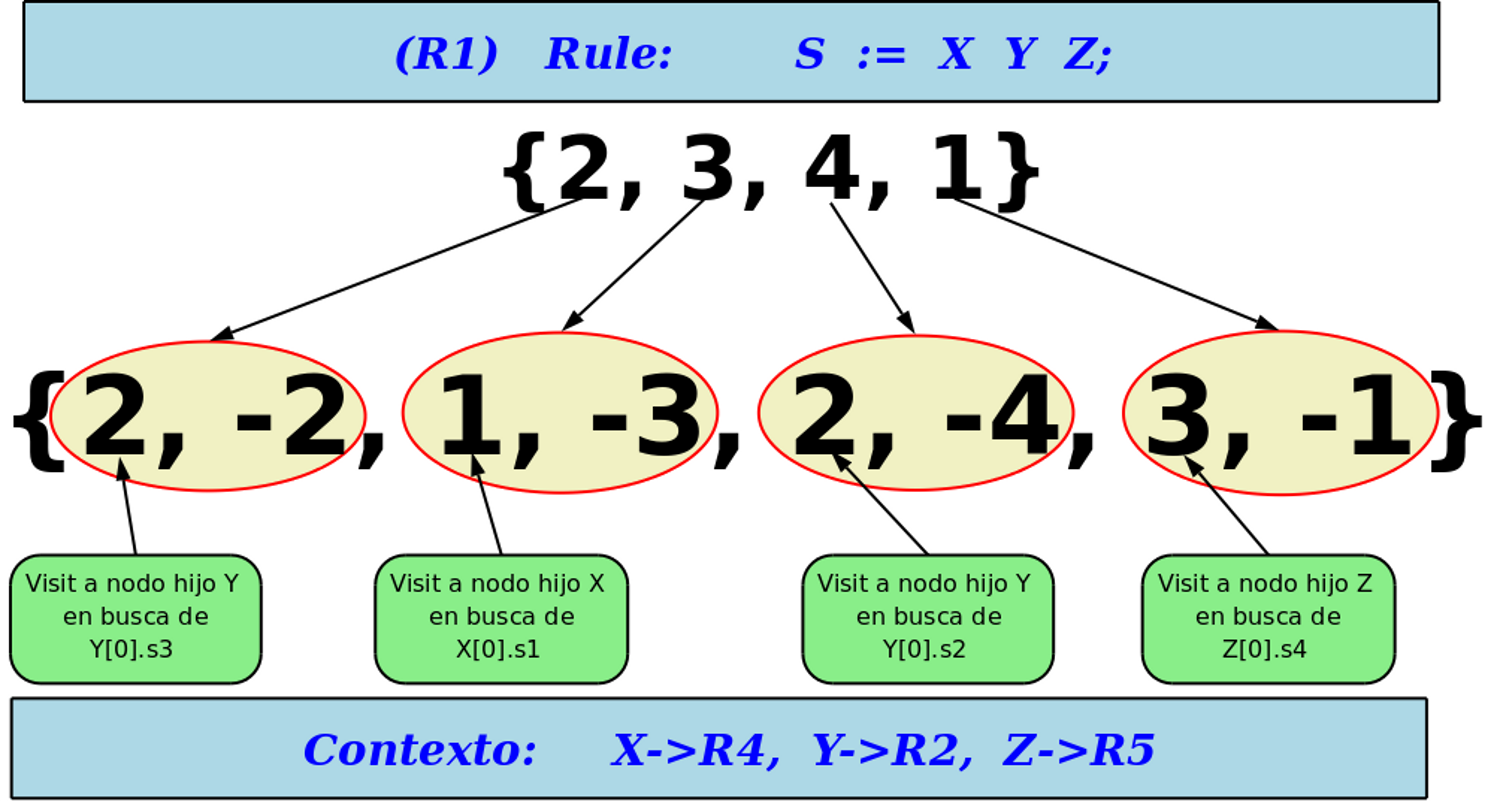
\includegraphics[width=300pt,height=160pt]{plan2seq.png}
\caption{\label{fig:resul_vis} Ejemplo de Secuencia de visita}
\end{figure}

Notar que para el cómputo de las secuencias de visitas totales, solamente basta con lanzar el algortimo, analizado anteriormente, para los planes iniciales\footnote{Los planes iniciales son aquellos que provienen de regla inicial.}. La explicación de esto se sustenta en las propiedades garantizadas con los chequeos en la gramática, principalmente la propiedad de alcanzabilidad. De esta forma, los planes iniciales lanzan los demás planes necesarios para el cómputo total de las secuencias.

\section{Generación de Código}
\label{sec:gencodigo}

La etapa final de \maggen\ esta dada por la generación de código para el evaluador estático. Como se ha analizado en el diagrama visto en la figura \ref{fig:disen}, esta etapa se realiza en el paquete ``Builder'', específicamente en el módulo \textbtt{Builder\_code}.

La etapa de generación de código produce dos archivos: \textit{interface} (.hpp) e \textit{implementación} (.cpp). En el apéndice \ref{append:agwuuyangcode} se puede observar el código generado para el ejemplo de Wuu Yang ya analizado durante todo este capítulo.

A continuación se abordarán algunas consideraciones sobre la generación de código en \maggen\ teniendo en cuenta lo observado en el apéndice.

Consideraciones de la clase:

\begin{description}
\setlength{\itemindent}{1em}
\setlength{\leftmargin}{1em}

\item [Atributos] la totalidad de los mismos tienen visibilidad privada.

\begin{lstlisting}[backgroundcolor=\color{white}, linewidth=9.5cm]
vector <Visit_sequence> v_seq;
vector <Order_rule>     contexts_rule;
vector <Plan>           eval_plans;
vector <Plan_project>   eval_plans_project;
vector <Rule>           rules;
\end{lstlisting}

Estos, son usados por los métodos del evaluador generado por \maggen. Se puede hacer una diferencia en el hecho de que, \textbtt{v\_seq} es usado directamente por el algoritmo de evaluación, en cambio los demás son usados por algoritmos previos a este. Cada uno de los tipos usados para estos atributos son definidos en otro módulo, el cual se analizará más adelante.

\item [Métodos] Es necesario distinguirlos según su visibilidad:

\begin{itemize}
\setlength{\itemindent}{1em}
\setlength{\leftmargin}{1em}
\item Privados:

\begin{lstlisting}[backgroundcolor=\color{white}, columns=fullflexible]
void add_plan(const Key_plan &k_plan, unsigned short index_order);
void add_plan_project(const Key_plan_project &k_plan_p, unsigned short index_order);
void compute_eq(int num_eq, struct Node *root);
void traverse(struct Node *node, unsigned short order);
void eval_visiter(struct Node *root);
\end{lstlisting}

Estos métodos son usados internamente por el evaluador generado por \maggen\ teniendo en cuenta lo siguiente:\\
\textbtt{compute\_eq} tiene la responsabilidad de invocar a los \textbf{compute} de cada ecuación y \textbtt{eval\_visiter} tiene la responsabilidad de los \textbf{visit} a nodos. Notar que, estos métodos trabajan sobre las secuencias de visita.

El método \textbtt{traverse} recorre el AST de entrada al evaluador y asigna a cada nodo un plan de evaluación\footnote{Los planes que asigna el método traverse son los generados estáticamente por \maggen.} y con ello una secuencia de visita correspondiente.

\textbtt{add\_plan} y \textbtt{add\_plan\_project} agregan planes y planes proyectados respectivamente, los mismos son usados en la inicialización del e\-va\-lua\-dor (constructor de clase).

\item Públicos:

\begin{lstlisting}[backgroundcolor=\color{white}, columns=fullflexible, linewidth=7cm]
maggen();
void print_visit_seqs();
void translates_visit_seqs();
void evaluator_mag(struct Node *root);
\end{lstlisting}

Estos, son los servicios públicos que ofrece el evaluador generado por \maggen. El método más importante, es \textbtt{evaluator\_mag}, el cual pone en funcionamiento el evaluador generado por \maggen. El parámetro tomado por el método representa la raíz del AST que se desea evaluar.

El constructor de clase\footnote{El nombre de la clase y por ende el del constructor de la misma depende de los parámetros con los cuales se invocó a \maggen\ (Ver capítulo \ref{chap:usos}).} realiza la inicialización de los atributos de la misma. Los valores de inicialización de los atributos son obtenidos por los cómputos de cada etapa de \maggen\ vistas en todo este capítulo.

Los dos métodos anexos, \textbtt{print\_visit\_seqs} y \textbtt{translates\_visit\_seqs} pueden ser usados para visualizar las secuencias de visita del evaluador. Los dos realizan la misma funcionalidad, pero muestran las secuencias de visita de manera diferente, como lista de valores o como secuencia de \textbtt{compute}, \textbtt{visit} o \textbtt{leave}.
\end{itemize}
\end{description}

Además de la clase, \maggen\ genera \textbtt{struct} para cada uno de los símbolos de la gramática y para cada uno implementa el método \textbtt{to\_string()} que se responsabiliza de como mostrar por pantalla cada símbolo, teniendo en cuenta sus atributos. Para más detalles analizar en el apéndice \ref{append:agwuuyangcode}, específicamente los \textbtt{struct} para los símbolos \textbtt{S, X, Y, Z}.

Los dos módulos analizados arriba, generados por \maggen, se apoyan sobre dos módulos más, que son anexados de manera estática por la herramienta, ellos son: \textbtt{Node.hpp} y \textbtt{Plan.hpp}.

Los mismos contienen definiciones de ``tipos'' y ``métodos'' necesarios por el el evaluador generado.

\subsection{Cabecera: \textbtt{Node.hpp}}

El tipo de datos nodo de un AST, se encuentra definido en este archivo. Los campos del mismo son:
\begin{items}
\item \textbtt{struct Node *parent:} referencia al nodo superior.

\item \textbtt{vector <struct Node*>\ childs:} listado de referencias a los hijos.

\item \textbtt{unsigned short rule\_id:} identificador de la regla que representa el nodo.

\item \textbtt{unsigned short visit\_seq\_index:} índice de la secuencia de visita que le corresponde al nodo para su evaluación.

\item \textbtt{unsigned short pos\_visit\_seq:} posición desde donde debe comenzar a recorrerse la secuencia de visita.
\end{items}

Además se encuentra su constructor y una funcionalidad para agregar hijos.

\subsection{Cabecera: \textbtt{Plan.hpp}}

Aquí se encuentran las definiciones de tipos necesarios para el evaluador:

\begin{items}
\item Orden de evaluación de ecuaciones:
\begin{lstlisting}[backgroundcolor=\color{white}, columns=fullflexible, linewidth=11.5cm]
typedef vector <unsigned short> Order_eval_eq;
\end{lstlisting}

\item Orden de evaluación de reglas (contexto):
\begin{lstlisting}[backgroundcolor=\color{white}, columns=fullflexible, linewidth=11.5cm]
typedef vector <unsigned short> Order_rule;
\end{lstlisting}

\item Clave para planes de evaluación:
\begin{lstlisting}[backgroundcolor=\color{white}, columns=fullflexible, linewidth=11.5cm]
typedef struct k_plan
{
    unsigned short  id_plan;
    unsigned short  plan;
    ...
} Key_plan;
\end{lstlisting}

\item Clave para planes de evaluación proyectados:
\begin{lstlisting}[backgroundcolor=\color{white}, columns=fullflexible, linewidth=11.5cm]
typedef struct k_p_project
{
    Key_plan        id_plan_project;
    unsigned short  node_project;
    unsigned short  index_ocurrence;
    ...
} Key_plan_project;
\end{lstlisting}

\item Secuencia de visita:
\begin{lstlisting}[backgroundcolor=\color{white}, columns=fullflexible, linewidth=11.5cm]
typedef vector <int> Visit_sequence;
\end{lstlisting}

\item Versión reducida de regla:
\begin{lstlisting}[backgroundcolor=\color{white}, columns=fullflexible, linewidth=11.5cm]
typedef vector <unsigned short> Rule;
\end{lstlisting}

\item Plan de evaluación:
\begin{lstlisting}[backgroundcolor=\color{white}, columns=fullflexible, linewidth=11.5cm]
typedef pair <Key_plan, unsigned short> Plan;
\end{lstlisting}

\item Plan de evaluación proyectado:
\begin{lstlisting}[backgroundcolor=\color{white}, columns=fullflexible, linewidth=11.5cm]
typedef pair <Key_plan_project, unsigned short> Plan_project;
\end{lstlisting}
\end{items}

\normalsize
